% Load the kaobook class
\documentclass[
	fontsize=10pt, % Base font size
	twoside=false, % Use different layouts for even and odd pages (in particular, if twoside=true, the margin column will be always on the outside)
	%open=any, % If twoside=true, uncomment this to force new chapters to start on any page, not only on right (odd) pages
	secnumdepth=1, % How deep to number headings. Defaults to 1 (sections)
]{kaobook}

% Choose the language
\usepackage[english]{babel} % Load characters and hyphenation
\usepackage[english=british]{csquotes}	% English quotes

% Load packages for testing
\usepackage{blindtext}
%\usepackage{showframe} % Uncomment to show boxes around the text area, margin, header and footer
%\usepackage{showlabels} % Uncomment to output the content of \label commands to the document where they are used

% Load the bibliography package
\usepackage{kaobiblio}
\addbibresource{intro-pubinv.bib} % Bibliography file

% Load mathematical packages for theorems and related environments
\usepackage{kaotheorems}

% Load the package for hyperreferences
\usepackage{kaorefs}

\graphicspath{{images/}{./}} % Paths where images are looked for

\makeindex[columns=3, title=Alphabetical Index, intoc] % Make LaTeX produce the files required to compile the index


\begin{document}

%----------------------------------------------------------------------------------------
%	BOOK INFORMATION
%----------------------------------------------------------------------------------------

\titlehead{Document Template}
\title[Public Invention]{Public Invention}
\author[RLR]{Robert L. Read}
\date{\today}
\publishers{Public Invention, a US public charity}

%----------------------------------------------------------------------------------------

\frontmatter % Denotes the start of the pre-document content, uses roman numerals

%----------------------------------------------------------------------------------------
%	COPYRIGHT PAGE
%----------------------------------------------------------------------------------------

\makeatletter
\uppertitleback{\@titlehead} % Header

\lowertitleback{
	\textbf{Disclaimer} \\
	You can edit this page to suit your needs. For instance, here we have a no copyright statement, a colophon and some other information. This page is based on the corresponding page of Ken Arroyo Ohori's thesis, with minimal changes.

	\medskip

	\textbf{Copyright 2021, Robert L. Read} \\
%%	\cczero\

	\medskip

	\textbf{Colophon} \\
	This document was typeset with the help of \href{https://sourceforge.net/projects/koma-script/}{\KOMAScript} and \href{https://www.latex-project.org/}{\LaTeX} using the \href{https://github.com/fmarotta/kaobook/}{kaobook} class.

	\medskip

	\textbf{Publisher} \\
	This book has not yet been printed. \@publishers
}
\makeatother

%----------------------------------------------------------------------------------------
%	DEDICATION
%----------------------------------------------------------------------------------------

\dedication{
  If you want to build a ship, don’t drum up the men to gather wood, divide the work, and give orders. Instead, teach them to yearn for the vast and endless sea.\\
	\flushright -- Antoine de Saint-Exupéry
}

%----------------------------------------------------------------------------------------
%	OUTPUT TITLE PAGE AND PREVIOUS
%----------------------------------------------------------------------------------------

% Note that \maketitle outputs the pages before here
\maketitle

%----------------------------------------------------------------------------------------
%	PREFACE
%----------------------------------------------------------------------------------------

\chapter*{Preface}

This is a draft work whose purpose is explain and promote Public Invention as a
movement and philosophy. My hope is to create a coherent and convincing work.
This work will likely be published electronically by Public Invention (the organization),
but we will also seek a print-publisher who is willing to keep the work open access.

-- Robert L. Read

%----------------------------------------------------------------------------------------
%	TABLE OF CONTENTS & LIST OF FIGURES/TABLES
%----------------------------------------------------------------------------------------

\begingroup % Local scope for the following commands

% Define the style for the TOC, LOF, and LOT
%\setstretch{1} % Uncomment to modify line spacing in the ToC
%\hypersetup{linkcolor=blue} % Uncomment to set the colour of links in the ToC
\setlength{\textheight}{230\vscale} % Manually adjust the height of the ToC pages

% Turn on compatibility mode for the etoc package
\etocstandarddisplaystyle % "toc display" as if etoc was not loaded
\etocstandardlines % "toc lines as if etoc was not loaded

\tableofcontents % Output the table of contents

\listoffigures % Output the list of figures

% Comment both of the following lines to have the LOF and the LOT on different pages
\let\cleardoublepage\bigskip
\let\clearpage\bigskip

\listoftables % Output the list of tables

\endgroup

%----------------------------------------------------------------------------------------
%	MAIN BODY
%----------------------------------------------------------------------------------------

\mainmatter % Denotes the start of the main document content, resets page numbering and uses arabic numbers
\setchapterstyle{kao} % Choose the default chapter heading style

\pagelayout{wide} % No margins
\addpart{The Joy of Public Invention}
\pagelayout{margin} % Restore margins

\chapter{“Invent in the public, for the Public.”}


Benjamin Franklin (1705-1790) did not patent the Franklin stove because
he believed it to be too useful an invention to legally encumber.
Benjamin Franklin has been
called ``The First American''\cite{Brands2000}, but I think of him as the
first Public Inventor.
If you read the autobiography of Nikola Tesla (1856-1943)
``My Inventions''\cite{Tesla1982},
you discover a devout public servant
(in a non-denominational sense), who certainly wanted to make
money but whose deepest motivation was to see human progress.
R. Buckminster Fuller (1895-1983) wrote extensively on the act of invention
as a moral act: nerve gas is bad, vaccines are good\cite{Fuller1981}.
Richard Stallman (1953-) articulated the principles of free software
and in so doing indirectly increased the wealth and well-being
of the planet tremendsouly\cite{Stallman2002free}.
This book is my attempt to extend and promote the work of
those inventors to create a stronger movement which we could
call Public Invention.

\nocite{laurel2001}

Invention is the most spectacular way to advance human progress.
It is odd that our politicians mostly ignore it.
The story of human history is largely a story of technological
advance careening foward from the stone age with
a speed which is inexorably, and frightentingly, building,
perhaps to a climax.
Those who believe it will end in a dark and terrible
destruction are not fools;
but that fate is not certain.
We as a planet can choose instead to build a bright future
in which humanity explores the universe together in peace.
This will happen only if we understand technology as the
powerful moral force that it is.

For the last 100 years, technological advance has been driven
by two engines: profit and academic research.
The modern emphasis of Universities of patenting research
and the governmental practice of subsidizing research which
is monopolized by for-profit firms has blurred the distinction.
Nations have long recognized the value of technology for
competiting with other nations via
war or mercantilism. Public Invention hopes to be a movement
that does not replace for-profit research and academic research,
but becomes a third engine. The motto of Public Invention
is ``Invent in the public, for the Public.''

\begin{marginfigure}[-5.5cm]
    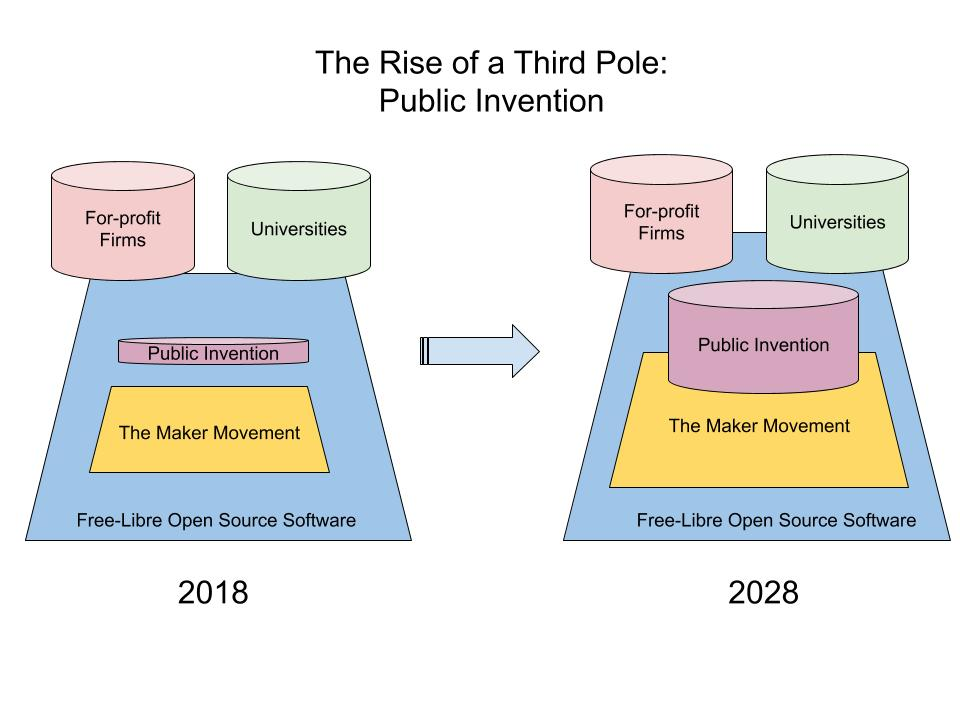
\includegraphics{figures/The_Rise_of_Public_Invention.jpg}
  \caption{The Rise of Public Invention as a Third Pole of Progress}
  \labfig{rise}
\end{marginfigure}

This means the Public Inventor does not seek monopolies in
the form of patents or other intellectual property but
gives an invention freely to the whole world without prejudice.
Anyone is free to use the invention, including for the purpose
of making a profit, but nobody is giving the privilege of
exclusive rights to it.

Buckminster Fuller made a clear distinction between what he
called ``killingry'', or weapons, and ``livingry''--that
which increase the good in the world. The Public Inventor
must not build weapons. This is impossible
to do perfectly.
Even a pillow can be used as a weapon. Nonetheless,
technologists are not relieved of the duty to invent
good things instead of bad things just because it is
intellectually difficult to decide what is good and what is bad.
The Public Inventor accepts this burden as does the best they can.

Benjamin Franklin said, ``We must, indeed, all hang together or,
most assuredly, we shall all hang separately.''
His wit was poignant because he meant the American revolutionary
leaders would indeed have swung from a British rope for treason
if the Revolutionary war had been lost.
But in 2021 his words still ring true. Buckminster Fuller
believed that humanity would either destroy itself or
have a bright, Star Trek-like future---there is no
middle ground.
We cannot continue to muddle along
taking weak action on global warming.
The COVID-19 pandemic has shown that we are all connected
in a most intimate way, whether we like it or not.
A disease incubated in my body may kill you, and vice versa.
Therefore the Public Inventor must at some level seek
the wealth and well-being of the whole world.
Narrow national chauvinism is no longer a useful or profitable
behavior.

We could define Public Invention simply as invention in the
public interest.
In that sense, it is closely related to humanitarian engineering.
Humantarian engineering requires a great deal of problem-solving,
innovation, and ingenuity. The distinction is that ``invention''
means something truly novel which has never existed before.
Public  invention values the truly novel, whereas
humanitarian engineering values the truly useful.

In the future, it will be common place for people to move freely
between
the three engines of for-profit firms, academic research,
and public invention.
Public invention will not replace the other two engines,
but augment them.
Public invention is a moral act, but it is not a moral duty.
Some people will want to be public inventors some of the time.

\chapter{The Joy of Public Invention}

Public invention takes the joy of invention and multiplies
it by the joy of helping others.
Making something truly new is a roller coaster ride
of emotions.
The inventor is frought with doubts.
Is the invention even possible?
Has someone done this earlier?
Am I too stupid to accomplish this?
Often a new idea creates innumerable frustrations.
The expensive equipment breaks at a critical momemnt.
There may be collaborators,
but there are no experts to turn to, because by definition
the invention has never been made before.
Despite all of the doubts and frustrations, or
perhaps because of them, the eventual progress, if it
comes, is an intense joy.

Comic books and movies have taken a grain of truth
and mythologized out of proportion to create the trope
of the lone inventor.
Most invention is done by teams.
Math, is, in the end, always social.
The joy of collaboration is part of the attraction
of being a public inventor.

Each of us is unique and has unique gifts to bring
to the table.
In a sense this is true in any part of life,
but it is a especially true in the act of invention.
Each of us has a different voice, even if we sing
the same song.
However, by definition, invention is making something
not just new in the sense of a variation of something
old, however unique, but new in the sense of breaking new
ground.
An invention is not yet another rose, it is a new kind of flower.
Even mediocre inventors such as myself are essential and necessary.
The mediocre work makes the great work easier.

Some people have an invention inside them that has to get out.
The seed of an idea planted in childhood may mature in the unconscious
until the time is right for it emerge.
Sometimes this is because of a persons great love of something.
We have all seen people enchanting by flying or
infatuated with light.
Some people can spend years entranced by a math problem.
The inventions may be useful, but unprofitable.
Some may even be potentially harmful. Certainly many men,
including myself, are fascinated by shooting things at
high velocity, such as in guns or rockets or bows
or catapults or water guns.
So long as the invention is not designed to harm,
the invention should be allowed to be born.
The line between invention and art is sometimes blurred.
The public inventor should support whimsical inventions
when a person has a strong desire to make it.

The public inventor should not make fakes or toys.
That is, the public inventor should make an object
whose value is that it is a miniature version of some
other object or like some other object which has intrinsic value.
Making a model of a beautiful airplane or ship is valuable
and fun, but it is not invention.
Making a fake starship is not invention.

However, the desire to make something new even if the
utility of the invention is hard to define should be
respected. This may be because it is artful, or may
have nothing to do with art, and its value may lie
in some other dimension.
Often, an invention that wants to be made that has
no clear purpose is a forerunner of something else
which cannot be conceived until the first invention
is real and can be held in hand.

To me, public invention is really about love---love of humanity,
of beauty, of the planet, of math, and of my fellow-inventors.
For some of us, the joys of learning, collaboration, invention,
and helping the world melded together in public invention
is the greatest joy we can imagine.
At the end of my life my proudest acheivement will be my children,
and my second greatest sense of joy will come from the
inventions I have given the world, however small they may be.

\chapter{Why it makes more sense than in the past}

Participation in public invention makes more sense with
each passing decade.
Although we suffer from inequity, in raw terms the world
is more abundant than ever before.
Commodities are cheaper.
Fewer people live in poverty.
The number of people who are financially able to take
a few months out of the work force to work on a public invention
project without compensation is higher than ever.
People are more generous than ever before.
The number of people who make a substantial income
essentially through patronage and tipping is probably
hire than ever before.
In a world of abundance, the need to make a profit
or to work relentlessly at a career should
become less imperative.

In America today, housing in large cities
and formal education are exceptions
to the general trend of things becoming cheaper and easier to obtain.
Participating in public invention is a powerful way to
obtain two things provided by a formal education:
the learning and reputation.

There are specific technical reasons certain kinds of
public invention are far more accessible than ever before.
In the first place, the internet has made many tutorials
and how-to documents available almost for free, from
how to use a soldering iron to very sophisticated academic
papers.
Secondly, the free software movement has made an ocean
of high quality software available.
Although it takes effort, almost any computing task can
now be accomplished without paying a cent for software.
It remains the case that some of the best scientific tools
do not yet have free-gratis alternatives of similar quality,
but the trend is incontrovertible: the cost of computing
is getting cheaper.
I'm writing and typesetting this book right now
using mostly free software tools.
This same software generally also makes it cheaper to
build new software.
Usually, software that it free
as in free-pizza is free as in free-speech---meaning that
anyone has the freedom to use it as a starting point for making
something new.
Software has limitations, but it is extraordinarily versatile.
It is the most general-purpose of all technologies. The fact
that it is free is a fundamental enabler of public invention,
because capital attracted based on expectations of profits is
not needed.

Hardware is more expensive, but has gotten dramatically
more accessible at a low price. 3D printers that cost USD\$300
can now do astounding things that were not even possible 30
years ago. Similarly, it is now possible to design printed
circuit boards on free software and have them fabricated
and very low costs, usually in about two weeks.
This capability augments the old-fashioned but still
useful soldering iron as a means of making sturdy circuits.
Of course the reduction in the price of computers, which
includes single-chip micro-contollers used in electronic
embedded systems is legendary.

Although I am weak on bio-hacking, I believe the same
expansion of capability at reasonable cost has occurred in
the word of biology and biochemistry.
Even optics, in the form of microscopy and teloscopy,
has seen major improvements.

Batteris and solar power have enabled deployment of
electronics portably and to remote off-the-grid locations.
Significant improvements in cameras, sonar, and other
sensors have also increased the sophistication available
at low cost.

(Create Matrix/Infographic of relative acceleration in fields.)

Although hardware cost remain a relative imepdiment
(see Chapter \ref{chp:material} for Public Invention's policy),
the combination of cheap hardware, free software, and
cheap connectivity has made innovation and invention much easier.
Sharing and publication of inventions is a
critical part of public invention, and that is also
now easier than it has ever been.

\chapter{Social Inventions}

Advances in ``hard'' inventions
have made public invention easier,
but ``soft'' inventions also play a role.
In particular, practices pioneered by the Free Software movement,
such as the way projects can self-organize and use
free software and hardware licenses, enable running a
project and sharing it freely.

The free and open-source software has developed a
set of cultural practices that allow teams to work together.
These include:
\begin{itemize}
\item cultural dissuassion of unnecssary splitting or ``forking'' of a project,
\item using recognition as an incentive for contributions,
\item using version control systems to manage contribtuions,
\item and using Agile software methods and big visible charts
  to manager work.
\end{itemize}
\sidenote{This is incomplete and others may have a better explanation that I can cite. In particular ``the Apache Way'' is worth citing here.}

An additional practice is that documenters and maintainers
are valued nearly as highly as software coders\sidenote{Cite Eric S. Raymond's ``How to be a Hacker''} here.
This is a cultural practice which is of paramount importance
to public invention as a movement.
Often, an invention has a kernel of math or ingenuity
that can only be created by someone well-versed in the
appropriate science and art.
However, public invention is a team sport.
Every contribution must be honored and valued.
In some sports, some positions naturally have more
opportunities for drama---the striker on a football team,
the pitcher on a baseball team.
But teamwork is essential to winning.
Those who manage projects, write documentation,
help with quality assurance and provide financing are
equally important.

The value of these cultural inventions cannot be overestimated.
But the creation of the GNU General Public License (GPL)
\sidenote{The work of the Richard Stallman and the Free Software Foundation in the creation of the GPL has inspired many other licenses
  practically created the field and practice now called ``free culture''. This goes far beyond the GPL, but we can use the GPL as the
  originating event for these other licenses.}
is of equal importance.
The GPL is brilliant in its simplicity: it gives the
user the right to modify and distribute a copyrighted work
and works derived from that a copyright work so long as
the distributor does not attempt to monopolize the works
and gives the derived work freely under the same terms.
The GPL and related Creative Commons licenses give
creators control over how their work is used.
In particular, they may choose to enable re-use, which
is the point of public invention.

There are also reciprocal licenses for hardware.
Hardware designs are not covered by copyright, and
so they are fundamentally different.
However, this is of no concern to the public inventor,
who as a matter a principle is giving away the invention
for the whole world to use freely.
It would be nice of those who take a device and made
improvements to it would contribute those improvements
back to the project and the world as the GPL forces
in software, but at present our legal structure for
doing this is weak.
We may, however, rely on the ``honor system'', which
can be astoundingly effective in practice.


\begin{itemize}
\item Practices pioneered by the Free Software Movement
\item  Internet community
\item Open Source Software paved the way with certain teachings
\item Projects need leaders
\item Projects run on the coin of acknowledgement
\item Maintainers and documenters are highly valued (quote ESR)
\item Licensing matters, but has been pioneered
\end{itemize}

\chapter{Imagining what it will be like}

\begin{itemize}
\item Infographic of the third pole
\item Smooth flow into and out of for-profit business
\item Profit becomes one of many tools
\item Easy to find a project that resonates
\item Easy to contribute something
\item But invention will always be hard, or it is not invention.
\item Replace vanity with gratitude
\item Imagining an altruism driven project landscape
\item Art and play in its place rising above infantilism
\item How to Achieve a World of Public Invention
\item An Ocean of Interesting, organized projects
\item A community of sharing
\item A means of getting of financial help
\item A means of getting mentorship
\item Judgement where it belongs
\end{itemize}

\chapter{Universal Salvation}

\begin{itemize}
\item Small is Beautiful
\item The road to the stars runs through villages and slums
\item None of us are free until all of us are free
\item Anthropomorphised money does not love poor people
\item Nor does it love rich people.
\item It wants to accumulate.
\item But people love people--we can motivate volunteers this way
\item We cannot live together on spaceship earth while we have grinding poverty
\item Cutting your own carbon footprint in isolation is of limited value compared to political action---yet we are “sold” such ideas.
\end{itemize}

\chapter{The Christian Point of View}

\begin{itemize}
\item Jesus never touched a soldering iron, but a soldier’s iron touched him.
\item Love your neighbor as yourself. (Matthew 22:35-40) -- the second half of the great commandment
\item The first part of the great commandment implies that all science is theology. By studying his works we study God; there can be no love without knowledge.
\item The second commandment requires sharing and egalitarianism.
\item If we are called to be little Christs, and God cares for every sparrow, then we must as well.
\item Talents must not be buried, and surely those of us who can be inventors have a talent: Matthew 25:14–30
Pauline comments:
 Whatever your hand finds to do, do with all your heart. (Ecclesiastes 9:10)
Each has separate gifts: (Ephesians 4:11-16)
\item We are made in God’s image; and is not God a Maker and Inventor and Mathematician?
\end{itemize}


\pagelayout{wide} % No margins
\addpart{How to Be a Public Inventor}
\pagelayout{margin} % Restore margins


\chapter{Practices}

\begin{itemize}
\item Motivate yourself through love of humanity, life, and knowledge
\item Publish early and often
\item Don’t seek patents
\item Publish your failures
\item Seek community
\item Help other Public Inventors
\item Ask for Help
\item Learn by doing
\item Failure in service to a big idea plants the seeds of success.
\end{itemize}

\chapter{What if you cannot be a Public Inventor?}

\begin{itemize}
\item Give moral support.
\item
  Give money in a way which is spiritually meaningful to you.
  \begin{itemize}
  \item A small amount given to a small project is incredibly impactful.
  \item People aren’t compensated, but paying for equipment has a multiplier effect
  \item It is psychologically important.
  \end{itemize}
\item Try to put yourself in a position that you can
  \begin{itemize}
  \item Educate yourself.
  \item Become financially sound---remove the desire for luxury
  \end{itemize}
\end{itemize}

\pagelayout{wide} % No margins
\addpart{Public Invention in the 2020s}
\pagelayout{margin} % Restore margins

\chapter{Public Invention 201: Essential Skills}

\chapter{The Technological Landscape}

I parts of this book will be read in the year 2100, but this chapter
will be obsolete.

\chapter{Selected Invention Ideas}

\pagelayout{wide} % No margins
\addpart{How Public Invention Operates}
\pagelayout{margin} % Restore margins

\chapter{The Invention Team Model}

\chapter{Sharing Immediately and Broadly}

\chapter{The Public Invention Licensing Policy}

\chapter{Why Public Invention is the best teacher, but is not an educational organization}

\begin{itemize}
\item People learn best by doing.
\item We don’t do exercises, fakes, or toys
\item Learning has an enormous social component
\item Learning is a precessional outcome of Public Invention activity
\end{itemize}


\chapter{Supporting Material Costs}
\label{chp:material}

\chapter{You Can Help}


\appendix % From here onwards, chapters are numbered with letters, as is the appendix convention



\chapter{Some more blindtext}

\blindtext

%----------------------------------------------------------------------------------------

\backmatter % Denotes the end of the main document content
\setchapterstyle{plain} % Output plain chapters from this point onwards

%----------------------------------------------------------------------------------------
%	BIBLIOGRAPHY
%----------------------------------------------------------------------------------------

% The bibliography needs to be compiled with biber using your LaTeX editor, or on the command line with 'biber main' from the template directory

\defbibnote{bibnote}{Here are the references in citation order.\par\bigskip} % Prepend this text to the bibliography
\printbibliography[heading=bibintoc, title=Bibliography, prenote=bibnote] % Add the bibliography heading to the ToC, set the title of the bibliography and output the bibliography note

%----------------------------------------------------------------------------------------
%	INDEX
%----------------------------------------------------------------------------------------

% The index needs to be compiled on the command line with 'makeindex main' from the template directory

\printindex % Output the index

\end{document}
